\documentclass{fizraport}
\authorA{Krzysztof Stasiowski}
\authorB{Joanna Binek}
\team{2}{2a}{1}

\topic{Moduł Younga}{11}{
Wyznaczenie  modułu  Younga metodą statyczną
za pomocą pomiaru wydłużenia drutu 
z~badanego metalu obciążonego stałą siłą. }
\carryOutDate{17.10.2018 r.}
\ftHandInDate{24.10.2018 r.}
\usepackage{csvsimple}
\usepackage{hyperref}
\usepackage{siunitx}
\begin{document}

\maketitle
\section{Wstęp teoretyczny}
\subsection{Moduł Younga}
Kiedy opisujemy zachowanie się ciała pod wpływem sił zazwyczaj posługujemy się
wyidealizowanym pojęciem bryły sztywnej, którego podstawowym założeniem jest
zachowanie względnych położeń poszczególnych części danego obiektu. W~wypadku gdy
potrzebujemy większej dokładności, lub gdy interesują nas odkształcenia danej bryły, możemy
zastosować prawo Hooke’a.

Prawo Hooke’a zakłada liniową zależność pomiędzy siłą jaka działa na~ciało a~jej
odkształceniem oraz, że~odkształcenie ciała w~wyniku siły następuje natychmiastowo i~
zatrzymuje się gdy siła przestaje oddziaływać na obiekt. Jest więc to~odkształcenie plastyczne
w~przeciwieństwie do~odkształcenia sprężystego w~którym ciało zmienia kształt po~usunięciu
siły rozciągającej. Warto zwrócić uwagę, że~prawo Hooke’a nie~bierze pod uwagę
wewnętrznej budowy ciała i~jest doświadczalną aproksymacją rzeczywistego nieliniowego
zjawiska przedstawionego na wykresie (\figref{fig:hook}).

\begin{figure}[!htb]
	\centering
	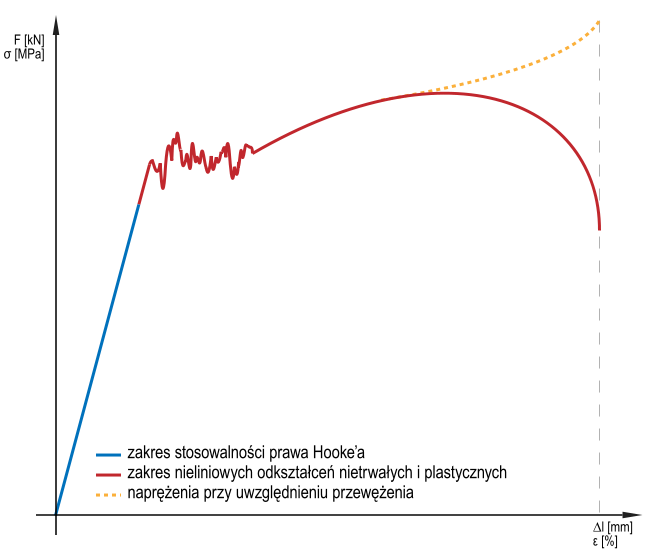
\includegraphics[scale=0.45]{wstep.png}
	\caption{Zależność obciążenia i~naprężenia od odkształceń dla stali z~zaznaczonym zakresem stosowalności prawa Hooke’a, źródło:  \url{http://www.wikipedia.pl}}
	\label{fig:hook}
\end{figure}
\pagebreak
Można więc je stosować tylko dla ciał o~niewielkiej plastyczności oraz lepkości, przy niewielkich siłach. Prawo~Hooke’a posiada
postać uogólnioną w~trójwymiarowej przestrzeni, ale w~tym doświadczeniu wektor
odkształcenia jest równoległy do~wektora siły więc zjawisko będziemy rozpatrywać
jednowymiarowo. W~takim wypadku prawo~Hooke’a dla pręta przyjmuje postać (\ref{eq:1}):

\begin{align}
    \Delta l = \frac{F \cdot l}{E \cdot S}
    \label{eq:1}
\end{align}

Gdzie $\Delta l$ jest zmianą długości pręta, $F$ przyłożoną siłą, $E$ to~moduł Younga,
charakterystyczny dla danego materiału, a~$S$ to pole przekroju poprzecznego. Prawo można
przedstawić też jako (\ref{eq:2}):

\begin{align}
    \sigma = E \cdot \varepsilon
    \label{eq:2}
\end{align}

Gdzie $ \sigma = \frac{F}{S}$ \si{[Pa]} i~oznacza naprężenie normalne; oraz $\varepsilon = \frac{\Delta l}{l} $ , czyli
normalne (prostopadłe do~przekroju poprzecznego ciała) odkształcenie względne.

Moduł Younga można interpretować jako naprężenie przy~którym długość ciała zostaje podwojona.
W~wypadku rzeczywistych materiałów prawo Hooke’a przestaje działać przy dużo mniejszych odkształceniach. Jednostką modułu Younga jest paskal $\si{[\frac{N}{m^2}]}$.


\section{Układ pomiarowy}
\begin{enumerate}
    \item Przyrząd do pomiaru wydłużenia drutu pod wpływem stałej siły (\figref{fig:uklad}), zaopatrzony w czujnik mikrometryczny do pomiaru wydłużenia drutu.
    \item Zestaw odważników
    \item Śruba mikrometryczna
    \item Przymiar milimetrowy
\end{enumerate}
\addplot[h]{urządzenie do~pomiaru modułu~Younga metodą~statyczną}{uklad}{uklad.png}{0.30\linewidth}

%\pagebreak
%\section{Zagadnienia Kontrolne}
\begin{enumerate}
    \item \par{Prawo Hooke'a - odkształcenie ciała pod wpływem, działającej siły jest proporcjonalne do tej siły. Współczynnik między naprężeniem wywołanym przez przyłożone siły odkształceniem nazywany jest modułem Young'a. Prawdziwe dla niedużych odkształceń i~tylko dla niektórych materiałów o ~pomijanie małej plastyczności. Można je wyrazić  wzorem:
    \[\frac{F}{S}=E\frac{\Delta L}{L}\]}
    \begin{itemize}
        \item[ ] $\Delta L$ - różnica długości
        \item[ ]  $L$ - pierwotna długość
        \item[ ]  $E$ - moduł Young'a
        \item[ ]  $S$ - powierzchnia przekroju poprzecznego
        \item[ ]  $F$ - siła działająca na ciało
    \end{itemize}
    Odkształcenie sprężyste - rodzaj odkształcenia, które ustępuje po usunięciu siły wywołującej to odkształcenie 
    \addtocounter{enumi}{1}
    \addtocounter{enumi}{1}
    
    \item Moduł Younga - wielkość opisująca sprężystość materiału przy pościąganiu i ściskaniu. Wyraża ona zależność względnego odkształcenia materiału do naprężenia jakie wnim występuje w zakresie odkształceń sprężystych wyraża się je w Pascalach $E=\left[\frac{N}{m^2}\right]=[\text{Pa}]$ 
    
    \item Co się stanie z Drutem po przekroczeniu jego granicy sprężystości?
    
    Po przekroczeniu granicy sprężystości rozpocznie się nieodwracalne odkształcenie drutu tj. po usunięciu siły działającej na drut pozostanie on trwale odkształcony.
    
    \item Dlaczego zmiany długości drutu s 2razy mniejsze od zmian długości  podawanych przez czujnik?
    Zmiany długości drutu ($d$) są 2 krotnie mniejsze od długości podawanej przez czujnik $D$, ponieważ są przyprostokątnymi dwóch trójkątów podobnych, których skala podobieństwa $k=\frac{A}{a}=2$, z powodu umiejscowienia drutu w połowie długości ramienia dźwigni.
    
    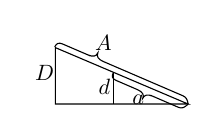
\begin{tikzpicture}[x=0.75pt,y=0.75pt,yscale=-0.4,xscale=0.4]
%uncomment if require: \path (0,446.25); %set diagram left start at 0, and has height of 446.25

%Straight Lines [id:da9313950171592851] 
\draw (430,100) --(270,32) -- (270,100)--(430,100)--(270,32)  ;


%Straight Lines [id:da6902289836929021] 
\draw (340,62) -- (340,100) ;
 ;


%Shape: Brace [id:dp7000132748697048] 
\draw   (430,100) .. controls (429.13,94.91) and (427.91,91.85) .. (423.62,90) -- (327.65,48.69) .. controls (321.53,46.06) and (319.39,42.6) .. (321.24,38.31) .. controls (319.39,42.6) and (315.41,43.42) .. (309.28,40.78)(312.04,41.97) -- (278.49,27.53) .. controls (274.2,25.68) and (271.14,26.9) .. (269.29,31.19) ;
%Shape: Brace [id:dp41634221637891644] 
\draw   (340,62) .. controls (337.43,66.49) and (338.65,69.55) .. (342.93,71.4) -- (368.93,82.63) .. controls (375.05,85.28) and (377.19,88.74) .. (375.34,93.02) .. controls (377.19,88.74) and (381.17,87.92) .. (387.29,90.56)(384.54,89.37) -- (418.08,103.86) .. controls (422.36,105.71) and (425.43,104.49) .. (430,100) ;


% Text Node
\draw (257,62) node [scale=0.8  ,opacity=1 ]  {$D$};
% Text Node
\draw (328,26) node [scale=0.8  ,opacity=1 ]  {$A$};
% Text Node
\draw (370,95) node [scale=0.8  ,opacity=1 ]  {$a$};
% Text Node
\draw (329,79) node [scale=0.8  ,opacity=1 ]  {$d$};

\end{tikzpicture}
%\pagebreak
\item Czym różni się definicyjny wzór na moduł Younga od wzoru roboczego:

Wzór definicyjny na moduł Younga:
\[E=\frac{\sigma}{\varepsilon} = \frac{\frac{F}{S}}{\frac{\Delta L}{L}} = \frac{FL}{S\Delta L}\]
Natomiast Wzór roboczy ma formę:
\[E=\frac{4L}{\pi d^2a} = \frac{L}{Sa}\]
gdzie $a$ jest współczynnikiem nachylenia prostej wyrażającej zależność $\Delta L(F)$, która z prawa Hooka powinna być linią prostą.
\end{enumerate}
\pagebreak
\section{Opis}

\subsection{Wykonanie ćwiczenia}
Wykonanie ćwiczenia rozpoczęliśmy od~zmierzenia długości drutu stalowego za~pomocą miarki o~niepewności pomiarowej 1mm.

Następnie zamocowaliśmy drut stalowy w~statywie za pomocą nakrętek. Po obciążeniu szalki dwoma odważnikami
kilogramowymi, zmierzyliśmy za pomocą śruby mikrometrycznej (o~niepewności pomiarowej 0.01 mm) średnicę drutu w~trzech różnych miejscach rozłożonych na całej jego długości.

Opróżniliśmy szalkę z~odważników, wyregulowaliśmy zamocowanie drutu tak, aby belka C dotykała końcówki czujnika mikrometrycznego (\figref{fig:uklad}) i~wyzerowaliśmy wskazania czujnika mikrometrycznego.

Po upewnieniu się, że czujnik mikrometryczny reaguje oraz wraca w położenie zerowe, przystąpiliśmy do serii pomiarów:
obciążaliśmy szalkę dokładając kolejne odważniki i~notując przy tym o~ile wydłuża się stalowy pręt.

Wykonaliśmy również czynności odwrotne~-~po~nałożeniu odważników o~maksymalnej wadze dla stalowego pręta zaczęliśmy je kolejno ściągać i~notować za każdym razem wskazanie czujnika. Wszystkie pomiary zapisaliśmy w~tabeli \tabref{tab:stal}

Analogiczną serię wykonaliśmy dla drutu mosiężnego i~pomiary zapisaliśmy w~\tabref{tab:mosiadz}.

\newlength{\colW}
\setlength{\colW}{2.2cm}
\begin{table}[thb]
\centering
\begin{flushleft}
Rodzaj materiału: stal\\
Długość drutu: $l$=1060 mm,~$u(l)$= 1 mm\\
Średnica drutu $d$: 0.29 mm,~0.28 mm,~0.29 mm\\
Średnica drutu średnia: $\Bar{d}=$ 0.29 mm,~$u(\Bar{d})=$ 0.01 mm\\
Współczynnik nachylenia wykresu:
$a_{stal}=0.01783$,~$u(a_{stal})=0.00054$\\
\end{flushleft}
\caption{Wyniki pomiaru drutu stalowego:}
\label{tab:stal}

\begin{tabular}{|r|r|r|r|r|}
    \hline
    \multirow[b]{4}{\colW}{ Masa odważników \\$[kg]$} & 
    \multirow[b]{4}{0.50\colW}{ Siła \\$[N]$} &
    \multirow[b]{4}{0.7\colW}{Wskazanie czujnika  $\uparrow $\\$[mm]$} &
    \multirow[b]{4}{0.7\colW}{Wskazanie czujnika  $\downarrow $\\$[mm]$} &
    \multirow[b]{4}{0.8\colW}{Średnie wydłużenie $\Delta l $\\$[mm]$}\\
    &&&&\\
    &&&&\\
    &&&&
    \csvreader[separator=semicolon, head to column names,]{tab2/tabelkaDlaStali.csv}{}
    {\\\hline \mass & \F & \up & \down & \mean}
    \\\hline
\end{tabular}
\end{table}
\begin{table}[thb]
\centering
\begin{flushleft}
Rodzaj materiału: mosiądz\\
Długość drutu: $l$=1610 mm,~ $u(l)$= 1 mm\\
Średnica drutu $d$: 1.19 mm,~1.19 mm,~1.19 mm\\
Średnica drutu średnia: $\Bar{d}=$ 1.19 mm,~ $u(\Bar{d})=$ 0.01 mm\\
Współczynnik nachylenia wykresu: $a_{mosiadz}=0.01979$,~$u(a_{mosiadz})=0.00085$\\
\end{flushleft}
\caption{Wyniki pomiaru drutu mosiężnego:}
\label{tab:mosiadz}

\begin{tabular}{|r|r|r|r|r|}
    \hline
    \multirow[b]{4}{\colW}{ Masa odważników \\$[kg]$} & 
    \multirow[b]{4}{0.50\colW}{ Siła \\$[N]$} &
    \multirow[b]{4}{0.7\colW}{Wskazanie czujnika  $\uparrow $\\$[mm]$} &
    \multirow[b]{4}{0.7\colW}{Wskazanie czujnika  $\downarrow $\\$[mm]$} &
    \multirow[b]{4}{0.8\colW}{Średnie wydłużenie $\Delta l $\\$[mm]$}\\
    &&&&\\
    &&&&\\
    &&&&
    \csvreader[separator=semicolon, head to column names,]{tab2/tabelkaMosiadz.csv}{}
    {\\\hline \mass & \F & \up & \down & \mean}
    \\\hline
\end{tabular}
\end{table}
\newpage
\section{Opracowanie wyników}
\subsection{Drut stalowy}
\begin{enumerate}
    \item Przedstawiliśmy na wykresie (\figref{fig:w1}) zależność średniego wydłużenia $\Delta l$ w~funkcji przyłożonej siły rozciągającej $F$, gdzie kolorem czerwonym zaznaczone są punkty które w~naszej ocenie odbiegają od prostoliniowego
przebiegu, a~niebieskim te punkty które braliśmy pod uwagę dopasowując do nich prostą metodą najmniejszych kwadratów. Wykorzystaliśmy do tego oprogramowanie komputerowe i~otrzymaliśmy prostą o~współczynniku nachylenia $a_{stal}=$\SI{0.01783}{\milli\metre\per\newton} z~niepewnością, $u(a_{stal})=\SI{0.00054}{\milli\metre\per\newton}$.
\addplot[c]{Wykres zależności średniego wydłużenia $\Delta l$ w~funkcji przyłożonej siły rozciągającej $F$}{w1}{Stal.pdf}{0.8\textwidth}

\item 
Wyliczony współczynnik nachylenia $a$ wykorzystaliśmy do~obliczenia modułu~Younga($E$) ze wzoru roboczego:(\ref{eq:young})
\begin{equation}
\label{eq:young}
    E = \frac{4l}{\pi d^2 a}
\end{equation}
\begin{equation*}
    E_{stal} = \frac{4l_{stal}}{\pi d_{stal}^2 a_{stal}}= \SI{899.93}{GPa} 
\end{equation*} %45,48 0329243

\item Z~kolei wyliczyliśmy niepewność modułu Younga $u(E)$ korzystając z~prawa przenoszenia
niepewności względnych ze wzoru dla trzech zmiennych:
\begin{equation*}
\footnotesize
\begin{split}
    u(E)&=\sqrt{\left (\frac{\partial E}{\partial a}*u(a)\right )^2+\left (\frac{\partial E}{\partial l}*u(l)\right )^2+\left (\frac{\partial E}{\partial d}*u(d)\right )^2}=\\
&=\sqrt{\left(\frac{-4*l}{a^2*\pi *d^2}*u(a)\right)^2+\left(\frac{4}{a*\pi *d^2}*u(l)\right)^2+\left(\frac{-8l}{a*\pi *d^3}*u(d)\right)^2}=\\
&= \sqrt{E^2\left (\frac{-u(a)}{a} \right )^2 + E^2\left (\frac{u(l)}{l} \right )^2 + E^2\left (\frac{-2*u(d)}{d} \right )^2}=\\
&= E\sqrt{\left (\frac{-u(a)}{a} \right )^2 + \left (\frac{u(l)}{l} \right )^2 + \left (\frac{-2*u(d)}{d} \right )^2} \\
\\
u_c(E) &= \SI{51.48} {GPa} 
\end{split}
\end{equation*}

\item Wyznaczyliśmy również niepewność rozszerzoną $U(E)$:
\begin{align*}
        U(E) &= k \cdot u_c(E) \\
        U(E) &= 2 \cdot  \SI{51.48}{GPa}  =  \SI{102.96}{GPa} 
\end{align*}
\end{enumerate}

\newpage
\subsection{Drut mosiężny}
\begin{enumerate}
    \item Przedstawiliśmy na wykresie(\figref{fig:w2}) zależność średniego wydłużenia $\Delta l$ w~funkcji przyłożonej siły rozciągającej $F$, gdzie kolorem czerwonym zaznaczone są punkty które w~naszej ocenie odbiegają od prostoliniowego
przebiegu, a~niebieskim te punkty które braliśmy pod uwagę dopasowując do nich prostą metodą najmniejszych kwadratów. Wykorzystaliśmy do tego oprogramowanie komputerowe i~otrzymaliśmy prostą o~współczynniku nachylenia $a_{mosiadz}=\SI{0.01979}{\milli\metre\per\newton}$ z~niepewnością, $u(a_{mosiadz})=\SI{0.00085}{\milli\metre\per\newton}$.
\addplot[c]{Wykres zależności średniego wydłużenia  $\Delta l$ w~funkcji przyłożonej siły rozciągającej $F$}{w2}{Mosiadz.pdf}{0.8\textwidth}

\item 
Wyliczony współczynnik nachylenia $a$ wykorzystaliśmy do~obliczenia modułu~Younga($E$) ze wzoru roboczego:(\ref{eq:young})
\begin{equation*}
    E = \frac{4l}{\pi d^2 a}
\end{equation*}
\begin{equation*}
    E_{mosiadz} = \frac{4l_{mosiadz}}{\pi d_{mosiadz}^2 a_{mosiadz}}=\SI{73.150}{\giga\pascal}
\end{equation*}

\item Z~kolei wyliczyliśmy niepewność modułu Younga $u(E)$ korzystając z~prawa przenoszenia
niepewności względnych ze wzoru dla trzech zmiennych:
\begin{equation*}
\footnotesize
\begin{split}
    u(E)&=\sqrt{\left (\frac{\partial E}{\partial a}*u(a)\right )^2+\left (\frac{\partial E}{\partial l}*u(l)\right )^2+\left (\frac{\partial E}{\partial d}*u(d)\right )^2}=\\
&=\sqrt{\left(\frac{-4*l}{a^2*\pi *d^2}*u(a)\right)^2+\left(\frac{4}{a*\pi *d^2}*u(l)\right)^2+\left(\frac{-8l}{a*\pi *d^3}*u(d)\right)^2}=\\
&= \sqrt{E^2\left (\frac{-u(a)}{a} \right )^2 + E^2\left (\frac{u(l)}{l} \right )^2 + E^2\left (\frac{-2*u(d)}{d} \right )^2}=\\
&= E\sqrt{\left (\frac{-u(a)}{a} \right )^2 + \left (\frac{u(l)}{l} \right )^2 + \left (\frac{-2*u(d)}{d} \right )^2} \\
\\
u_c(E) &=  \SI{3.34}{\giga\pascal}
\end{split}
\end{equation*}

\item Wyznaczyliśmy również niepewność rozszerzoną $U(E)$:
\begin{align*}
        U(E) &= k \cdot u_c(E) \\
        U(E) &= 2 \cdot 3.34 = \SI{6.68}{\giga\pascal}
\end{align*}
\end{enumerate}

\pagebreak
\section{Porównanie wyników}
\begin{table}[htb]
\centering
\caption{Porównanie wyników z~wartościami tablicowymi} \label{tab:endTable}
\newlength{\CW}
\setlength{\CW}{3.7cm}
\begin{tabular}{|c|c|c|c|}
\hline
  \multirow{3}{*}{Materiał} &
  \multirow{3}{\CW}{Moduł Younga $E$ - Wzór roboczy(\ref{eq:young})\\ $\si{[\giga\pascal]}$}&
  \multirow{3}{\CW}{Niepewność rozszerzona\\ $U(E)$\\ $\si{[\giga\pascal]}$ }&
  \multirow{3}{\CW}{Moduł Younga $E$ - Wartość tablicowa\\$\si{[\giga\pascal]}$ } \\&&&\\&&&\\ \hline
  
Stal    & 899.93 & 102.96  & 210-220 \\ \hline
Mosiądz & 73.15 & 6.68 & 90-110 \\\hline

\end{tabular}
\end{table}


\section{Wnioski}
Wyliczone przez nas wartości modułu Younga  nie są w~granicach niepewności rozszerzonej zgodne z~wartościami~tablicowymi.
Biorąc pod uwagę wartości uzyskane podczas pomiarów  w~\tabref{tab:mosiadz}~i~\tabref{tab:stal}, przyczynami tak dużej rozbieżności między obliczonymi przez nas wynikami, a~wartościami oczekiwanymi mogą być:
\begin{itemize}
    \item fakt, że druty po zamocowaniu w urządzeniu były jeszcze krzywe, co sprawiało, że część pracy ciężaru została spożytkowana na ich wyprostowanie
    \item niebezpośrednie obciążenie drutów
    \item ogólny stan drutów, ich pozaginanie i~wiek
\end{itemize}


\end{document}